\chapter{Literature Study}\label{ch2}

The aim of this proposed project is to develop a method to detect images created by a style-based generator architecture for generative adversarial networks in a set of artificial images (generated images of human faces contained in the StyleGAN dataset) and authentic images (Flickr-Faces-HQ dataset of human faces used as a benchmark for StyleGAN). Before the aim of the project can be satisfied, a literature study is required on neural networks and StyleGAN. The basic structure of neural networks and the different types of neural networks will be researched and discussed in context with the StyleGAN technology, and the detection of StyleGAN generated images. Current detection methods will be investigated and examined to evaluate their workings and relevancy towards a StyleGAN application. In conclusion, all knowledge acquired from the literature study will be used when creating the artefact to detect StyleGAN generated images.

\section{Neural Networks}

In recent times, neural networks have been regarded as a fast-growing field offering powerful tools for most types of problem-solving \citep{Albawi}. The increased use results from the neural network's capabilities to function even with large data sets as input effectively. Therefore, a study into neural networks is required as it is a tool to use in the detection of StyleGAN generated images because of the large datasets accompanying StyleGAN. 

\subsection{History of Neural Networks}

Artificial intelligence is a modern growing field within information technology rooted in historical discoveries leading to new advances. Artificial intelligence has been in the development stages since the mid-20th century. However, early on, most advances made in artificial intelligence were developed in mathematics and computational model theory \citep{Mueller1995}.

Warren McCulloch and Walter Pitts initialised the now big field of artificial intelligence when they proposed a new general theory in information processing that artificial neurons can mimic the neurons present in the human brain \citep{Mueller1995}. \cite{Mueller1995} also notes that the neurons Warren McCulloch and Walter Pitts proposed were more simplified than biological neurons and still promised reliable computational power. The artificial neuron that could be implemented in a network to mimic a single neuron cell in the human brain and mimic the whole brain as a network is the foundation of early artificial intelligence and machine learning theory.

The next significant advance in this field came in the 1960s by researchers Caianiello and Rosenblatt. This advance resulted from focusing on two aspects of Artificial Neural Network's (ANN): 1\textsuperscript{st} being the aim to mimic their biological counterparts in their design and the 2\textsuperscript{nd} is that different structures proposed different advantages \citep{Mueller1995}. This difference of structure leading to a difference of perception is present in nature, where mammals all possess a biological brain, but the shape and network design allow mammals to think differently based on their specific computational needs\citep{Mueller1995}. Rosenblatt coined the differing structure of ANN's as the perceptron of the network, and in modern artificial intelligence theory, the perceptron is called the perception of the neural network.

The historical, theoretical initialization of neural networks is the foundation of modern neural networks. Modern neural networks' development focuses on practical applications in modern times. Neural networks are still relatively new in artificial intelligence, with theory founded in historical mathematics

\subsection{The Function of Neural Networks}

Neural networks are present in most forms of biological computation. For example, the human brain is a neural network of neurons that allow us to compute our daily tasks. An ANN mimics the human brain in its structure \citep{Krenker2011}. Like a human brain thinking through the impulses sent and received between biological neurons, an ANN sends and receives input and output through the artificial neurons in the network \citep{Krenker2011}. The neurons that form the network allow neural networks to imitate a biological brain's basic structure and computation. 

An artificial neuron is a single node within a neural network. This neuron is an independent node residing in a neural network that receives data and applies the neuron's mathematical model to this input. The output is the result of a calculation and the operation of activation and deactivation of the node.

\cite{Krenker2011} states that the neuron structure consists of three separate stages. The first stage applies the weight to the input with multiplication. The second stage is a sum function of all the previous stage weights and biases applied to the initial input. The final stage of the artificial neuron determines if the neuron should be activated or deactivated \citep{Krenker2011}. Artificial neurons activated or deactivated artificially enable the neural network to "think" and adaptively apply its computation on inputs.

\begin{figure}[!htbp!]%
\centering
\fbox{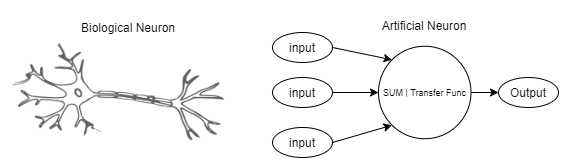
\includegraphics[width=0.95\textwidth]{img/f4.png}}%
\caption{Biological Neuron and Artificial Neuron \cite{Krenker2011}}%
\label{fig:4}%
\end{figure}

Figure 2 shows the similarities between the biological neural network and the ANN. The basis of biological neural network for the design foundation of an ANN is 

The set of neurons functioning together to form a network is called a neural network. In a biological brain, the whole cellular neurons connected in the brain and artificial intelligence are the ANN with the artificial neurons working together. ANN's are capable of processing information of real-world problems that requires a more complex approach because they can distribute their neurons in a non-linear, parallel structure \citep{Krenker2011}. Multiple neurons simultaneously are the neural network structure, and neurons do not have to flow their output into the next.

Figure 3 illustrates a primary ANN with connected neurons that mimics the structure of connected biological neurons connected inside the human brain. Each neuron within the structure of the ANN in Figure 3 can be compared to a human single brain cell in the biological brain structure. The artificial neuron present in the network only apply basic computational calculation on the data, and as output, the node only activated or deactivated itself.

\subsection{Neural Network Learning Paradigms}

Neural networks can learn in different ways, and these differences pose their respective advantages and disadvantages—the manner of learning in a neural network the network's learning paradigm.  The three different learning paradigms for neural networks used in the training of neural networks are supervised learning, unsupervised learning, and reinforcement learning \citep{Krenker2011}. The learning paradigms for neural networks are also specific to the type of data the network use in training. Concerning image classification and computer vision, only two of the three learning paradigms apply, namely supervised learning and unsupervised learning \citep{OShea2015}. Different neural network topologies use different learning paradigms. The specific choice of learning paradigm is essential in the implementation of the detection method of StyleGAN images. 

\subsubsection{Supervised Learning}

The supervised learning paradigm sets the parameters of the neural network based on the training data set it receives. The critical difference in supervised learning is that the input data is labelled before training the neural network \citep{Krenker2011, OShea2015}. The already labelled input is then compared to the output of the neural network to determine its error and accuracy. Training is applied to the network based on comparing the output the network created against the labelled input. If this paradigm is applied to the StyleGAN image detection problem, the training set of data consist of a set of images of human faces and a set of StyleGAN generated images. This input training set requires parameters or labels that identify a single image as either a human face or a StyleGAN generated image. The prediction made by the neural network will then be validated against these know classifiers on the images, and training will take place based on how the neural network predictions compare to the valid identifiers. In deep neural networks, supervised learning also deals explicitly with the labelled data. The advantages of supervised learning applied in deep neural networks such as CNN and GAN are that training can be conducted without initial knowledge about the differences between two different data inputs. The fallback to this advantageous method is that when there is outlying data present within the dataset, An image of a dog in the set of authentic images, the training can overstrain the boundary of decision \citep{Alzubaidi2021}.

The supervised learning paradigm is subdivided into two separate fields determined by the specialisation required while the neural network learns in the training phase. Semi-supervised learning and self-supervised learning selection are determined by how the input data is labelled to provide the neural network with information \citep{Zhai}. For a supervised learning approach, when aiming to identify StyleGAN generated images, the subsections of supervised learning must be evaluated in context to this project. 

Semi-supervised learning is a good choice of training algorithm if the input data is both labelled and unlabelled. In most cases, the learning algorithm assumes the label of input data if the data originated from the same distribution \citep{Zhai}. In the case of analysing StyleGAN images, the 2 labelled data sets are authentic images and generated images. When selecting a semi-supervised learning algorithm, the initial labels in the dataset must be standardised, and the data set is then altered that only a portion of the labels is kept with the data set. The algorithm treats the rest of the dataset as unlabelled data \citep{Zhai}. Semi-supervised learning was based initially on different neural network architectures, and one prominent algorithm used was the GAN that is also the basis of StyleGAN. An advantage of semi-supervised learning is that it applies inductive learning through generalisation, mapping the inputs to the outputs classify the data that have the most significant impact on the output of the network. 

Self-supervised learning uses only the unlabelled data to formulate mundane tasks within the network. It is commonly used to label datasets that have no classification of data \citep{Zhai}. Self-supervised learning algorithms can be implemented on the StyleGAN identification utilizing it labelling the dataset. The input dataset can then be a combination of StyleGAN generated images and authentic images that the self-supervised learning algorithm will then aim to solve by labelling the data as either generated by StyleGAN or is a unique actual human image. One problem with implementing this learning algorithm is that the data set containing StyleGAN images and authentic human faces are very similar. Differences are minimal between the two images, and Self-supervised learning might struggle to distinguish between the two different images, and miss labelling might occur. 

\subsubsection{Unsupervised Learning}

The difference with the unsupervised learning paradigm compared with supervised learning is that with unsupervised learning, the data does not have the added information that can aid the neural network in determining its correctness of prediction. The unsupervised learning paradigm entails learning based on a set cost function and minimising the goal's cost \citep{Krenker2011}. With a StyleGAN application, this paradigm will not necessarily help the neural network to learn effectively. This inefficiency results from an image's initial problem, either an actual image or a fake image. And a cost function to how fake an image might not necessarily lead to the neural network deciding that the image was generated using StyleGAN. This particular case is substantiated by the artefacts embedded in StyleGAN images. In specific cases, the neural network can receive a StyleGAN generated image close to an actual image with only one unique artefact created by the StyleGAN inefficiency. The cost function might still pass that image as an actual image, yet a person will quickly identify the artefact in the image with ease. More on StyleGAN artefacts will follow further in the StyleGAN analysis.

The different learning paradigms discussed each poses their own set of advantages and disadvantages. In the context of identifying StyleGAN generated images, supervised learning could be the chosen learning paradigm, more specifically semi-supervised learning, because of the two labels present in images used to train the neural network. On the other hand, self-supervised learning will not be used because of the minor differences between a StyleGAN image and an actual human face image.

\subsection{Hot and Cold Learning}

Hot and Cold learning is one of the most straightforward approaches to determining the optimal weights for machine learning problems. In a StyleGAN problem hot and cold learning will be randomly guessing the initial hyper parameters and  changing them in training to increase the accuracy of the neural networks prediction. 

Hot and cold learning is the process of increasing and decreasing the weights after a prediction and then training the model again. In theory, the continuous repetition of this process will lead to an error value of 0. Based on the increased or decreased error value, the changes in weights should either increase or decrease. \citep{Trask2019} However, hot and cold learning is not efficient. A developer must repeat a process manually numerous times until they finally stumble on a perceived perfect combination of weights. This implementation also does not ensure that optimal values are found. A developer might start by changing a parameter to its "\textit{optimal values}” and then changing another to the previous and ultimately closing in on a false optimal set of parameters.

Hot and cold learning is a simple form of machine learning that is not optimal and might not get the best values for training a model. Hot and Cold learning falls behind because its implementation may lead to false positives where changes in the hyper parameters leads to reduced prediction values and show that the data is optimal yet there may be an even better set of parameters. However, it is useful when implemented on minor scope problems and in the initialization in developing a neural network where hyper parameter optimization can improve the mode further. Hot and cold learning will aid in the understanding of hyperparameters and how it connects to the machine learning model and improvements in training.

\subsection{Neural Network Architecture}

The structure in which the artificial neurons are presented within a neuron network is the neural network architecture. There are multiple different neural network architectures with different benefits and disadvantages in specific practical applications. StyleGAN is a generative adversarial neural network that applies specific styles to create a new unique image \citep{Karras2019}. A technique of identifying neural network generated images such as those generated from ProGAN, StarGAN and Deepfakes focused on the shared base convolutional neural network architecture of these technologies \citep{Wang}. Therefore GANs and convolutional neural networks are identified as relevant architectures that require deep analysis in this study to ensure a thorough understanding of these architectures that will be interacted with in detecting StyleGAN images.

\subsubsection{Convolutional Neural Network}

Neural networks perform exceptional at identifying patterns hidden in different large datasets, but specific neural network architectures perform better than others when implemented to detect these patterns within specific data set consisting of different data types \citep{Liu2017}. Convolutional neural networks (abbreviated as CNN) commonly used for computer vision are great neural network architecture options for identifying patterns in image datasets \citep{Albawi, Yosinski2015}. When trying to detect StyleGAN generated images, a large dataset containing images generated through StyleGAN and a large dataset containing images of humans will be used to train the neural network. A CNN could be an appropriate neural network architecture to use in the detection method because of the specific large image dataset required to solve this problem.

CNN's are similar to the more basic ANN's, with the only difference being the advances a CNN has towards image classifications and pattern recognition within computer vision \citep{OShea2015}. In a CNN, the primary neuron within the network improves throughout learning, and the network still takes a single weight and apply it throughout. CNN's consists of layers that interact with the raw image data and declassify it into raster data where subsequent layers preside over the fragmented raster's consecutively. CNN's are chosen for image application because ANN's struggle with the computation power needed when attempting image classification \citep{OShea2015}.

\begin{figure}[H]%
\centering
\fbox{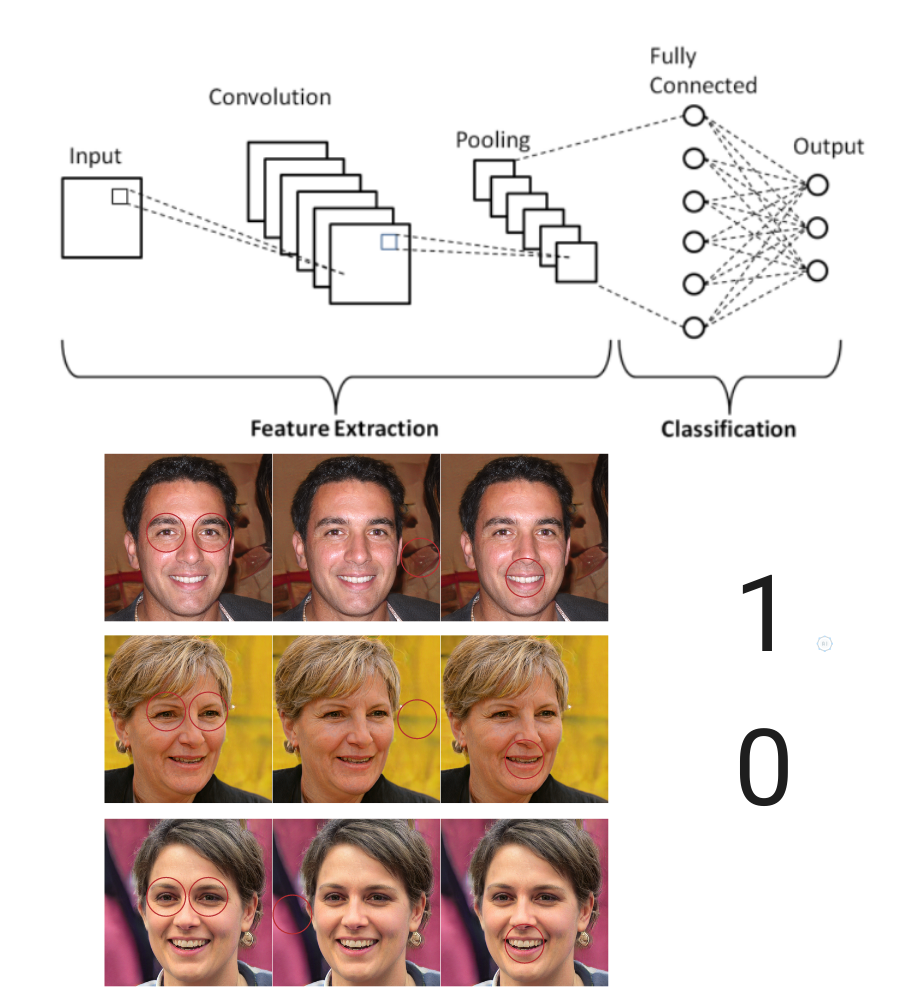
\includegraphics[width=0.5\textwidth]{img/f9.png}}%
\caption{Possible Architecture of CNN applied to the StyleGAN problem \citep{Karras2019, OShea2015}}%
\label{fig:9}%
\end{figure}

The network architecture of a CNN is divided into three dimensions categorised as the convolutional layer, pooling layer and fully-connected layer \citep{OShea2015}. The dimensionality created by the stacked layers sets CNN's apart from ANN's in image classification. The first layer in a CNN distinguishes it from the standard ANN and produces improved performance when it is implemented for image classification.

When the input is passed through this layer, the convolution applies various filters on the data to activate two-dimensional maps \citep{OShea2015}. These 2D maps determine if features are present in the image based on pixels activated when filtered on the activation maps. The convolutions within this network can get large in dimensionality, and the pooling layer is responsible for reducing the complexity of the calculated data \citep{OShea2015}. The function of the pooling layer to reduce the dimensionality of the network can be detrimental to the data because any dimensional reduction in the architecture of the NN further reduces the data dimension simultaneously. Finally, neurons gather the data directly from nodes in the previous layer and, without connecting the preceding layers, conclude the neural network \citep{OShea2015}.

\begin{figure}[H]%
\centering
\fbox{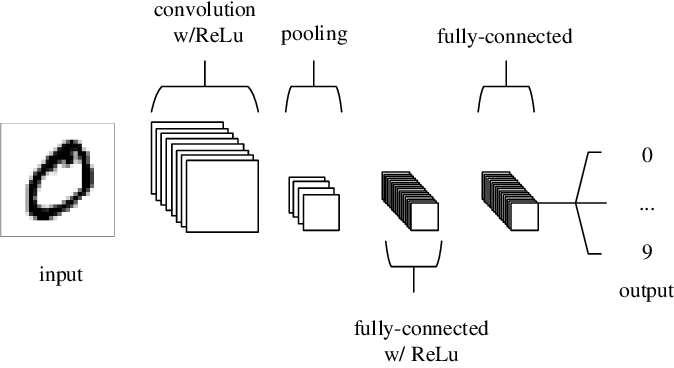
\includegraphics[width=0.8\textwidth]{img/f5.png}}%
\caption{CNN used in the classification of digits \cite{OShea2015}}%
\label{fig:5}%
\end{figure}

Figure \ref{fig:5} visualizes the hidden convolution layer, pooling layer, and the fully connected layers within a CNN. Various iterations of the layers pose different advantages and disadvantages in a practical application.

The benefit when using a CNN on an image processing problem is the improved accuracy in detecting objects within the image \citep{Albawi, Alzubaidi2021}. The activation maps present in a CNN enables the neural network to robustly identify objects within an image through the localisation of the raster data. CNN share weight between its parameter, and this reduces the number of required nodes in training. The reduction in training nodes improves CNN generalisation and reduces overfitting created by the training process. The localisation and object detection of CNN requires extensive calculations, and the process is computationally expensive. This drawback means that without the necessary graphical processing hardware, the training of the CNN will take a long time compared to most other neural networks \citep{Alzubaidi2021}

\subsubsection{Generative Adverserial Networks}

Competition increases the performance of sports athletes, students, and businesses \citep{Burguillo2010,Hays2009,Medvedev2005}. Neural networks can train themselves with the appropriate datasets as identified earlier. With the analogy that a neural network aims to mimic the human brain in its structure, the assumption can be made that competition might increase a neural network's performance. This assumption that competitive neural networks competing against one another led to the formulation of GANs \citep{Creswell2018}.

GAN's use a discriminator and generator to produce two neural networks competing against one another \citep{Creswell2018}. The result of pitting two networks to compete against each other leads to the network being able to improve itself more effectively and further increase application possibilities with these types of networks \citep{Goodfellow2014}. The generator constantly tries to fool the discriminator and the discriminator, in turn, try to identify when its input originated from the generator. 
The generator can be characterised as a criminal trying to falsify identification documents and the discriminator as a customs officer checking a passport. The criminal constantly tries to fool the customs officer. When he succeeds, the officer remembers the fake passport he missed in his identification of fake passports, and the process starts again. The officer learned from his mistake and can in future detect fake passports better. When the criminal fails, the process restarts and similar to the officer the criminal also learns from his mistakes and adapts how he generates fake documents \citep{Goodfellow2014}. The generator constantly creates, and the discriminator constantly describes. This cat and mouse game of fooling and detection in training is how a GAN evolves into the robust networks present in the field of fake images created by neural networks.

\begin{figure}[H]%
\centering
\fbox{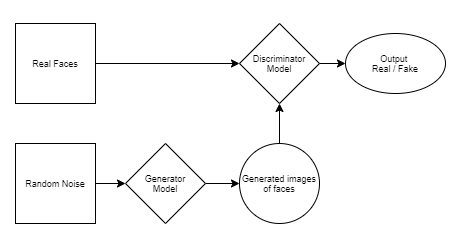
\includegraphics[width=0.8\textwidth]{img/f6.png}}%
\caption{GAN architecture adapted from \cite{Creswell2018}}%
\label{fig:6}%
\end{figure}

A demonstration of how the structure of a GAN allow the discriminator to be critical of the generator output is evident in Figure \ref{fig:6}. The advantage brought on by this neural network architecture is the improved data processing performance. The GAN can process images with sharper resolution than the standard ANN that require images with reduced sharpness for model integrations \citep{Goodfellow2014}. The main disadvantage of implementing GAN is increasing complexity to keep the generator and discriminator synchronised while training the models. 

StyleGAN and StyleGAN2 are GANs with an improved generator that applies specific "styles" on images, and the combination leads to the generation of new images \citep{Karras2019,Karras2020}. A convolutional GAN is a GAN implemented where the generator creates images with convolutional neural network architecture. This combination of the GAN checking against itself while creating images with the architecture of CNN enables improvisation in image generation \citep{Karras2019,Wang}.

\subsection{Activation Functions in Neural Networks}

Activation functions is a crucial part of neural networks and their processing capabilities. Without the presence of activation functions in the nodes of a neural network, the learning of the network will be reduced and the maps between the input and the output will not reach the required complexity. In this literature study an analysis on activation functions, why they are necessary and the different types of activation functions available must be conducted.

\subsubsection{Activation functions are crucial for neural network learning}

Activation functions are the processes on the nodes within the layers of neural networks that allow information to be derived from the data in specific ways. An activation function determines in what way the node will set itself on/off and allow its weight to influence the output of the network. Activation functions are used in an ANN to transform the input signal on a node to the output signal and sequentially add the output of the previous layer to the input of the next layer \cite{sharma2017}.

The inputs and weights are calculated first and then before the output is sent to the next layer the activation function is applied on the node \citep{sharma2017}. Accuracy within neural networks can fluctuate greatly and is influenced by the number of layers within the network and the types of activation functions used. The types of activation functions within the neural network however has a more significant influence on the accuracy of the prediction of the neural network \cite{sharma2017}. There is no clear way to determine the best number of layers a neural network architecture must consist of, but there is a clear consensus between data scientists that a minimum of two layers must be used \cite{sharma2017}.

In neural networks, there are different types of activation functions but the most common set of these functions is the non-linear activation functions \citep{sharma2017}. In neural network activation functions, there are boundaries present and these boundaries describe the type of activation function a specific approach consist of, in a linear activation function this boundary is linear \citep{sharma2017}. Because of these linear boundaries in linear activation functions, the neural network will only be able to change its perception of the data in linear increments. The problem however faced with these activation functions is that real-life scenarios and problems the errors present consist of non-linear characteristics \citep{sharma2017}. Therefore data scientists opt for non-linear activation functions over linear activation functions in their functional neural network implementations.

In the development of the artefact the use of non-linear neural networks will ensure that complex information will be processed from the initial dataset. By adding non-linear activation functions to the neural network the output and steps toward the output will be non-linear in the result. 

The most important aspect of using activation functions is that the functions are differentiable so that backpropagation optimization can be implemented. When backpropagation can be implemented with the use of gradient descent will the neural network have the capability of calculating the errors and losses based on the calculated weights its uses within its layers \citep{sharma2017}.

\subsubsection{Different types of activation functions}

Different types of activation functions can be used and implemented on the layers within the neural network. The type of activation function that can be used depends on the data set and properties present in the data, and the output required from the data. As an example for binary image classification the layers in the network will have to consist of ReLU activation layers, yet the final output layer must be a Sigmoid activation layer.

\begin{table}[H]%
\caption{Different Activation Functions in Neural Networks \citep{sharma2017}}
\label{tabl:actfnn}
\centering
\small
\begin{tabular}{cccccc}
\hline
\\ Linear & Sigmoid & Tanh & ReLU & SoftMax & ExpoLU \\
\hline
\end{tabular}
\end{table}

In the review on activation functions it is apparent that activation functions is a crucial aspect of neural networks and the successful output that neural network can present. Activation functions have a bigger impact on the prediction accuracy of a neural network than the number of layers present within the neural network. There is still some guessing involved into which functions will result in the best accuracy predictions of the neural network but to some degree, there is a clear consensus as to what function will work best with specific types of data. Image classification is improved with the use of ReLU functions throughout the neural network layers and a Sigmoid activation functions as it finals output layer.


\subsection{Summary}

With the evaluation of CNN and GAN, an understanding of neural networks in the context of the aim of this project was conducted. CNN provides enhanced capabilities in the generation and classification of image data. While GAN provides specific alterations to images and specialized focus on own output validation and improvement. For the neural network training on a dataset containing authentic images and StyleGAN generated images, supervised learning is the appropriate choice. The architecture and learning paradigms choices for neural networks should be influenced by the type of application and datasets used within training, and because of this, a CNN neural network with semi-supervised learning will be used in the development of the project's artefact.

\section{StyleGAN}

StyleGAN brought new developments in applying styles on images and changing these styles to morph images into new unique style based changes \citep{Karras2019}. Fraudsters are empowered to better create fraudulent identities by applying these styles to images of faces. A fraudster can use StyleGAN to apply styles on their faces to change how they are perceived at checkpoints and more. StyleGAN still introduced advantages to the field; however, the detection of these images is necessary in today's media-centric world. The technology of StyleGAN generated images must first be understood to create a successful implementation technique to detect the generated images.

The StyleGAN addition to the vast sets of different neural networks implemented on different problems originated sequentially with the advances made in the fields of convolutional neural networks and GANs. Because of the computational advances of CNN discussed earlier StyleGAN improved in its generation of new images. StyleGAN2 further improved on this by reducing artefacts brought on in combining styles using the GAN from StyleGAN \citep{Karras2020}.

\subsection{StyleGAN Architecture}

The structure of StyleGAN differentiates it from normal GANs and allows for the combination of "styles" to create new images of non-existing humans \citep{Karras2019}. StyleGAN initializes with an insertion of the base image and input parameter of what styles need to be applied to that image, such as age, sex, and race. Applying all these parameters in the neural network leads to an image being created that changes the styles in the base image. StyleGAN architecture altered the architecture of the generation model to allow for more control over generating with different styles.

Figure \ref{fig:7} illustrates the original StyleGAN network architecture and compares the StyleGAN architecture to the architecture of a traditional GAN. The mapping of the styles added to the architecture of traditional GANs present and a clear indication of how StyleGAN can apply the styles within images can be seen.

\begin{figure}[H]%
\centering
\fbox{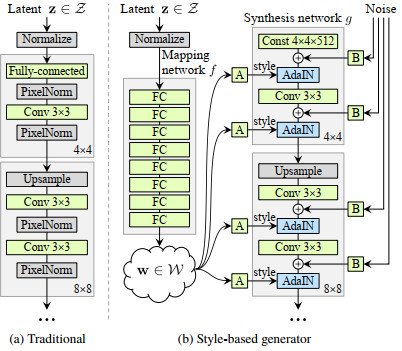
\includegraphics[width=0.7\textwidth]{img/f7.png}}%
\caption{Network architecture of StyleGAN vs Traditional GAN's \citep{Karras2019}}%
\label{fig:7}%
\end{figure}

Differences in authentic images and StyleGAN images are minimal. The most noticeable differences are the artefacts that StyleGAN generates due to deficiencies within the StyleGAN technology. These artefacts vary from rain-drop blotches in images to hair strands not showing realistic definition \citep{Karras2020}. In the second iteration of StyleGAN, the artefacts were addressed with minor improvisations but remain present in StyleGAN2 images \citep{Karras2020}.

\begin{figure}[!htbp!]%
\centering
\fbox{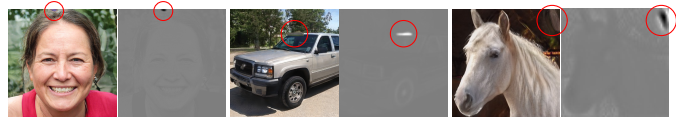
\includegraphics[width=0.95\textwidth]{img/f8.png}}%
\caption{Artefacts present in StyleGAN generated images adapted from \cite{Karras2020}}%
\label{fig:8}%
\end{figure}

Figure \ref{fig:8} illustrates artefacts present in StyleGAN generated images. This water drop effect present in these images could be more accessible for humans to identify than for a neural network due to the generalization of raster data \citep{Karras2020}.

\subsection{Detection of CNN Generated Images}

To detect StyleGAN generated images, the discriminator of the initial neural network can, in theory, be isolated and used to detect images created by the generator. The generator recurrently aimed to fool the discriminator, and the discriminator constantly adapted to the generator \citep{Karras2020}. The isolation of the discriminator is an invalid approach to detection because of how learning takes place within the creation of the StyleGAN network and when stoppage occurred in the training phase of the initial technology. The discriminator stops training before the generator, and thus an isolated discriminator will not be able to detect the output of the improved generator. In StyleGAN, the discriminator is not available to the public and to isolate it would require retraining of the GAN with the initial datasets of Flickr Faces images. A basic technique of supervised training to detect CNN generated images was implored by the researchers, and their results proved successful in detecting generated CNN images \citep{Wang}.

\begin{table}[!htbp!]%
\caption{Results of \cite{Wang} detecting various CNN's generating images}
\label{tabl:1}
\centering
\small
\begin{tabular}{ccc}
\hline
CNN-image generator & Detection accuracy of \citep{Wang}\\ 
\hline
ProGAN & 98.8\% \\
StyleGAN & 99.6\% \\
BigGAN & 66.4\%\\
CycleGAN & 88.7\%\\
StarGAN & 87.3\%\\
Deepfake & 58.1\%\\
\hline
\end{tabular}
\end{table}

\cite{Wang} proved that by employing a neural network to train labelled images as either real or faked, CNN-generated images could be detected. Table 1 results from their application of different image generation or changing neural networks. The success that \cite{Wang} achieved demonstrated that a semi-supervised neural network can detect CNN-generated images. Therefore a simple neural network approach is validated, and in the context of detecting StyleGAN images, a similar approach will be taken.

The basic architecture and structure of the generator of StyleGAN discussed previously gives more understanding of how StyleGAN can create such precise replication images of human beings. The success of a previous form of detection was evaluated, and StyleGAN images can be detected. By evaluating the work conducted by \cite{Wang}, a primary neural network with semi-supervised training is identified as a solid foundation for further detecting StyleGAN generated images.

\section{Summary}

Through this literature study, research and developments surrounding StyleGAN, neural networks, and different network architectures and learning paradigms were evaluated and discussed. CNN can create or detect images utilizing the strong computational power provided. GAN can change or initially create derived images, and StyleGAN can implement further control over the changes in the generated images. The types of neural networks involving StyleGAN and other surrounding technologies were evaluated, and an approach was discovered. A simple neural network utilizing semi-supervised learning will train on StyleGAN generated images and authentic images of human faces contained in the Flickr faces dataset will it be possible to detect these generated images as initially discovered by \citep{Wang}. The knowledge gained throughout this literature review will be used to develop the artefact to detect StyleGAN images. The development of the final artefact that detects these images will form the third chapter in this project